\documentclass[tikz,border=3pt]{standalone}
\usetikzlibrary{arrows.meta,calc}
\begin{document}
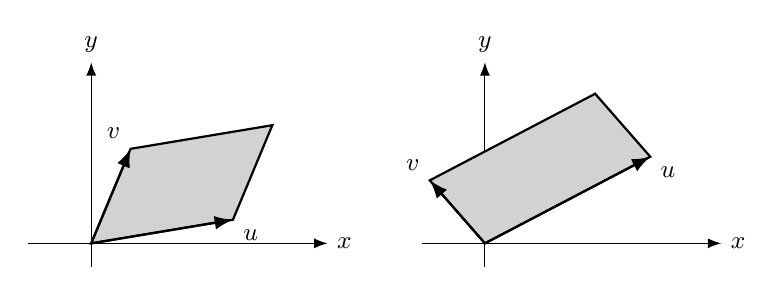
\begin{tikzpicture}[>=Latex, font=\small]
  \draw[->] (-0.8,0) -- (3,0) node[right] {$x$};
  \draw[->] (0,-0.3) -- (0,2.3) node[above] {$y$};
  \fill[gray!35] (0,0) -- (1.8,0.3) -- (2.3,1.5) -- (0.5,1.2) -- cycle;
  \draw[thick] (0,0) -- (1.8,0.3) -- (2.3,1.5) -- (0.5,1.2) -- cycle;
  \draw[->, thick] (0,0) -- (1.8,0.3) node[below right] {$u$};
  \draw[->, thick] (0,0) -- (0.5,1.2) node[above left] {$v$};

  \begin{scope}[xshift=5cm]
    \draw[->] (-0.8,0) -- (3,0) node[right] {$x$};
    \draw[->] (0,-0.3) -- (0,2.3) node[above] {$y$};
    \fill[gray!35] (0,0) -- (2.1,1.1) -- (1.4,1.9) -- (-0.7,0.8) -- cycle;
    \draw[thick] (0,0) -- (2.1,1.1) -- (1.4,1.9) -- (-0.7,0.8) -- cycle;
    \draw[->, thick] (0,0) -- (2.1,1.1) node[below right] {$u$};
    \draw[->, thick] (0,0) -- (-0.7,0.8) node[above left] {$v$};
  \end{scope}
\end{tikzpicture}
\end{document}
